\section{Trading Environment}
We build a trading environment compatible with Open AI Gym \cite{brockman2016openai} that serves two primary goals. The first objective is to translate domain-specific inputs into state/reward as inputs to the RL model. The second goal is to build the portfolio from the output of the RL model, the action.
\begin{figure}[ht]
  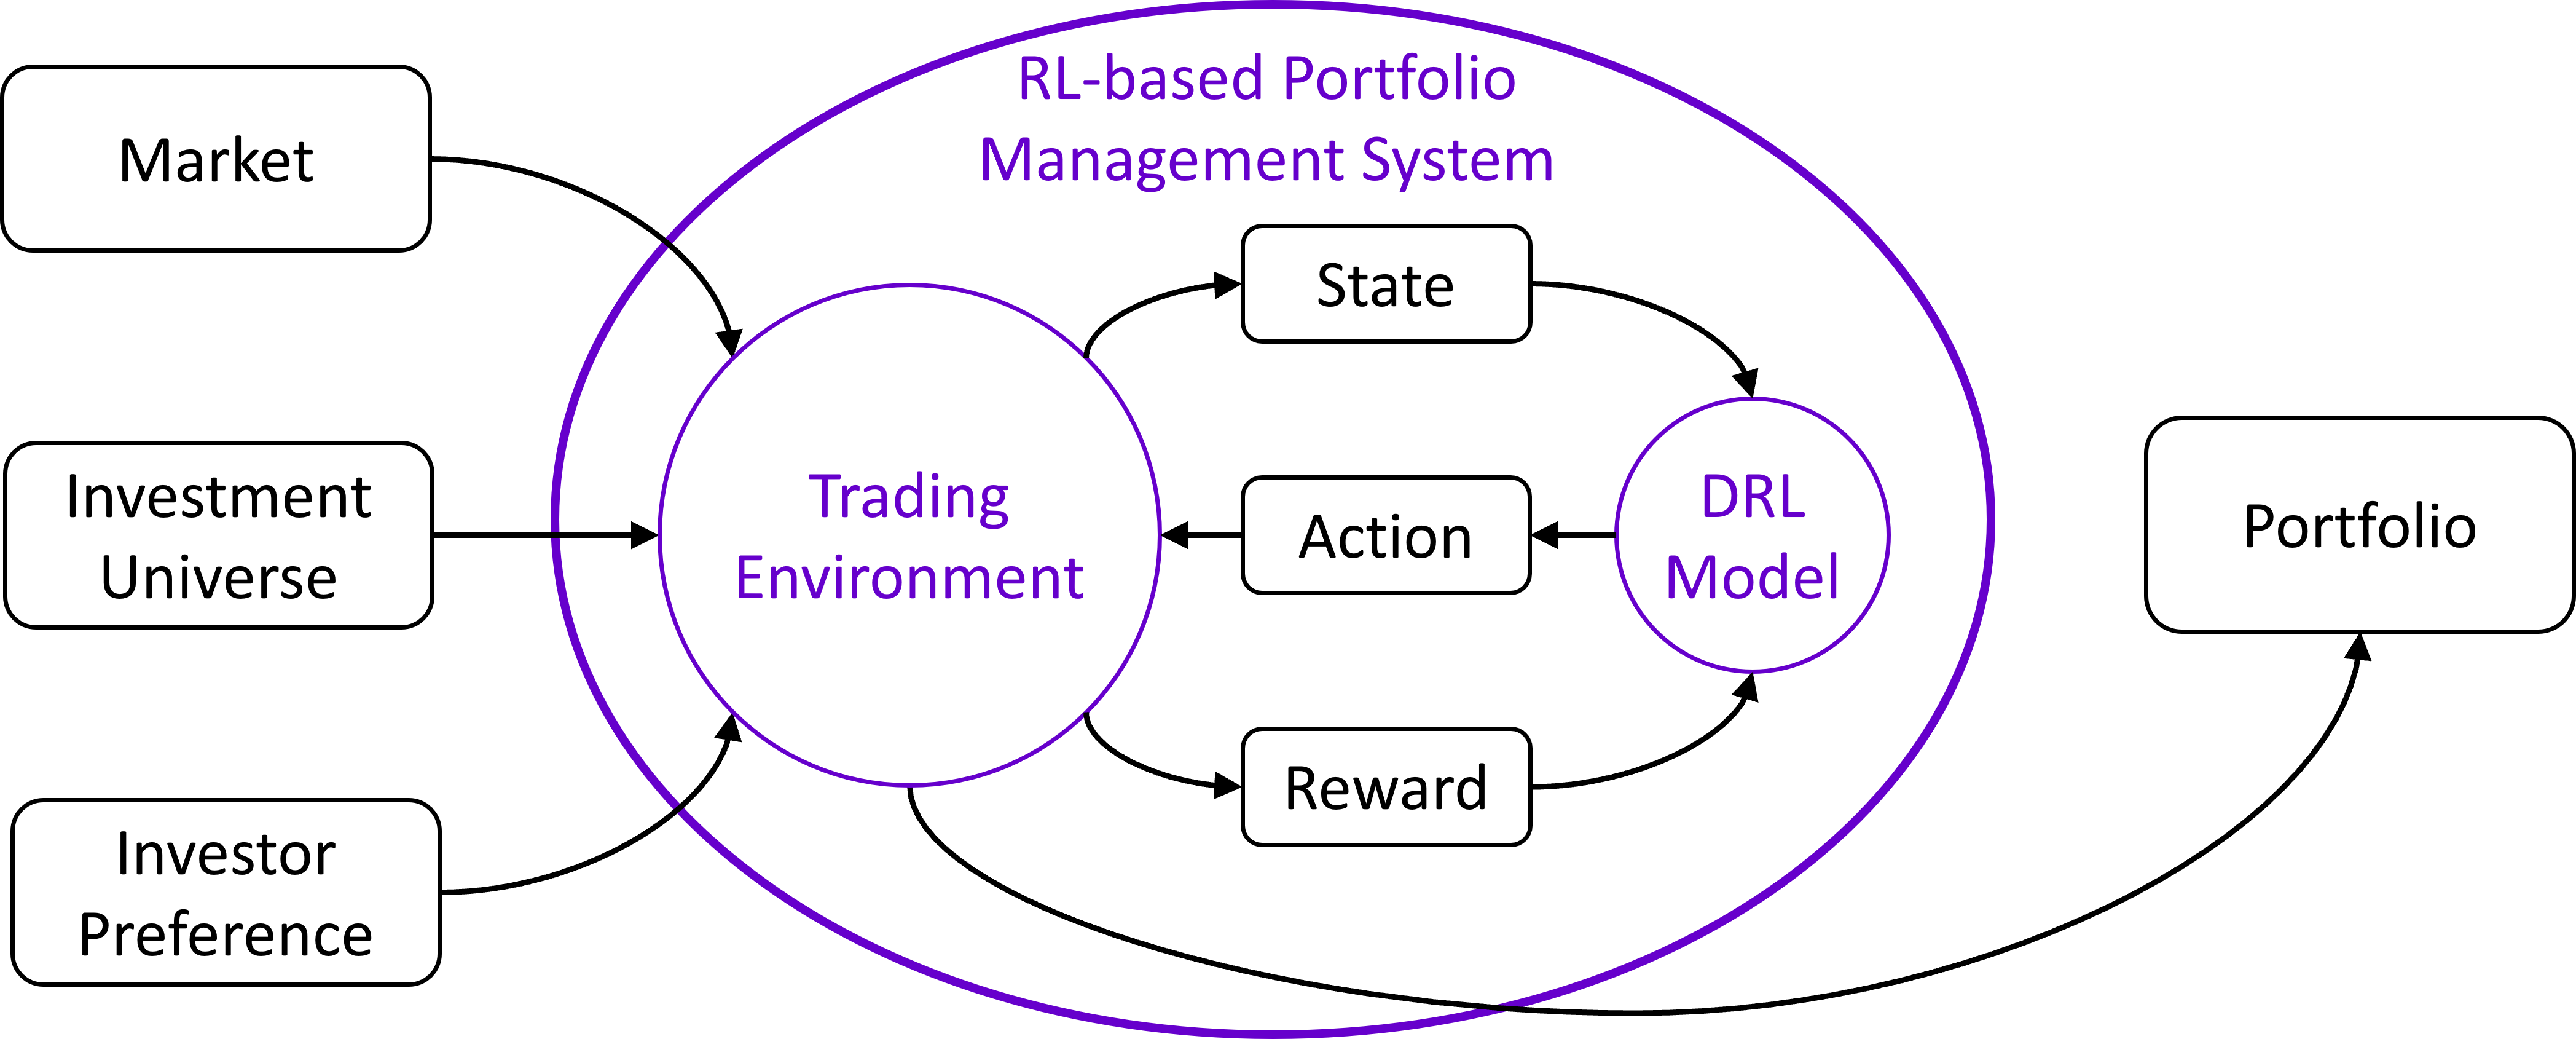
\includegraphics[width=15cm]{images/trading_environment.png}
  \caption[Trading Environment] { The trading environment uses market, investments, and investor Preference as input and transfers them into state and reward as inputs to the RL model. The environment will also build the portfolio base on the action from the RL model.}
  \label{fig:trading_environment} 
\end{figure}
\par
The observable state S is an n dimension vector space of real numbers between -1 and 1, where n is the number of features.
\[
    S = \{ {s \in \mathbb{R} | -1 \leq s \leq 1 } \} ^n
\]

\par
The reward R is a real number without any other constraint.
\[
    R \in \mathbb{R}
\]

\par
The trading environment contains few components, State Extractor, Portfolio Builder, Trading System, and the Reward Provider to archive its objectives.

\subsection {Feature Extractor}
The feature extractor extracts states from the features. 
The first step is to normalize the input features to mean 0 and standard division \(\sigma_{state}\),
\[
    f^{'}_{i,t} = \frac{\sigma_{state} \times   (f_{i,t} -  \overline{f_i})}{\sigma_{f_i}}
\]

We observed that the difference in performance between training and validation is significant in terms of Compound annual growth rate (CAGR) during our experiment. We assume overfitting is one of the causes, so we include noise in Gaussian distribution with mean 0 and variance \(\sigma_{noise}^2\) \(\mathcal{N}(0,\sigma_{noise}^2)\) into the state as an approach of data augmentation to reduce overfitting.
\[
    s_{i,t} = f^{'}_{i,t} + \mathcal{N}(0,\sigma_{noise}^2)
\]
The validation results improved significantly after adding noise to the states. We also experiment with the model with pure noise. Both training and validation have trivial improvement. This proves that the performance of features and noises results from the combined effort of both noises and the features, not noises alone.
\begin{figure}[ht]
  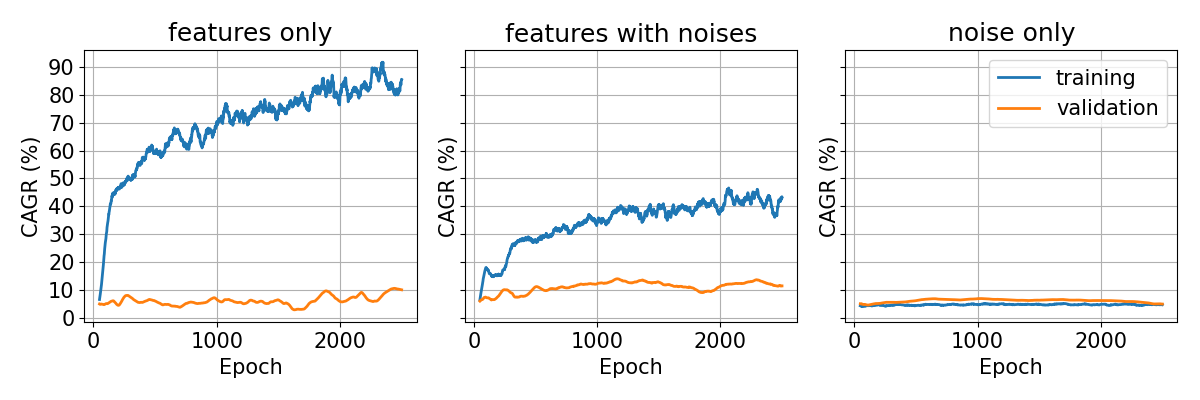
\includegraphics[width=15cm]{images/compare_noise.png}
  \caption [Comparison of features/noise] {Comparison of using features only, features with noises, and noises only as states in terms of training and validation CAGR (moving average 50 epochs)}
  \label{fig:noise_diagram}
\end{figure}

\subsection {Portfolio Builder}
The portfolio builder builds the portfolio from the investible universe and the action from the RL model.
The portfolio F contains no short position and is an m dimension vector space of weights w, a real number between 0 and 1. , where m is the number of investments in the investment universe. Wealth will all be in the form of investments, so the sum of the weights will equal 1.
\[
    F = \{ {f \in \mathbb{R} | 0 \leq f \leq 1 } \} ^m,
    \\
    \sum_{i=1}^m {f_i} =1
\]
We distribute the weight based on the action proportionally.
\[
    F_i = \cfrac{a_i}{\sum a} 
\]
where \(F_i\) is the weight for \(i^{th}\) investment, \(a_i\) is the  \(i^{th}\) action, m is the total number of investments in the investible universe. 
\subsection {Trading System}
The trading system measures performances of the given portfolios, including MDD, CAGR, profit, and wealth. These performances will be the input to calculate the reward or evaluate the performance of the system. 
\subsection {Reward Provider}
The Reward Provider provides rewards based on the performances of the portfolio and investor preference. We first introduce a reward equal to the profit p, with a penalty upon negative profits exceeding the given absolute value threshold \(\theta\). 
\[
p_t = \frac{w_t-w_{t-1}}{w_{t-1}}
, 
R_t = 
\begin{cases}
    p_t,&\text{if  }p_t > -\theta\\
    2p_t - \theta ,&\text{if  }p_t \leq  \theta
\end{cases}
\]
Where \(R_t\) is the reward, \(p_t\) is the profit and \(w_t\) is the wealth on given t.
\\
On all threshold \(\theta\) given, the result shows unstable improvement in MDD. We observed that the optimization goes too well during training and generates a tiny amount of negative profits; therefore, these negative profits have minimal penalty effect on the model parameters.
\\
We than apply the plenty on both positive and negative profits. This increase the stabliltiy signifantly.
\[
R_t = 
\begin{cases}
    2p_t - \theta,&\text{if  }    $$|p_t|$$ > \theta\\
    p_t - \theta ,&\text{if  } $$|p_t|$$\leq  \theta
\end{cases}
\]



\begin{figure}[ht]
  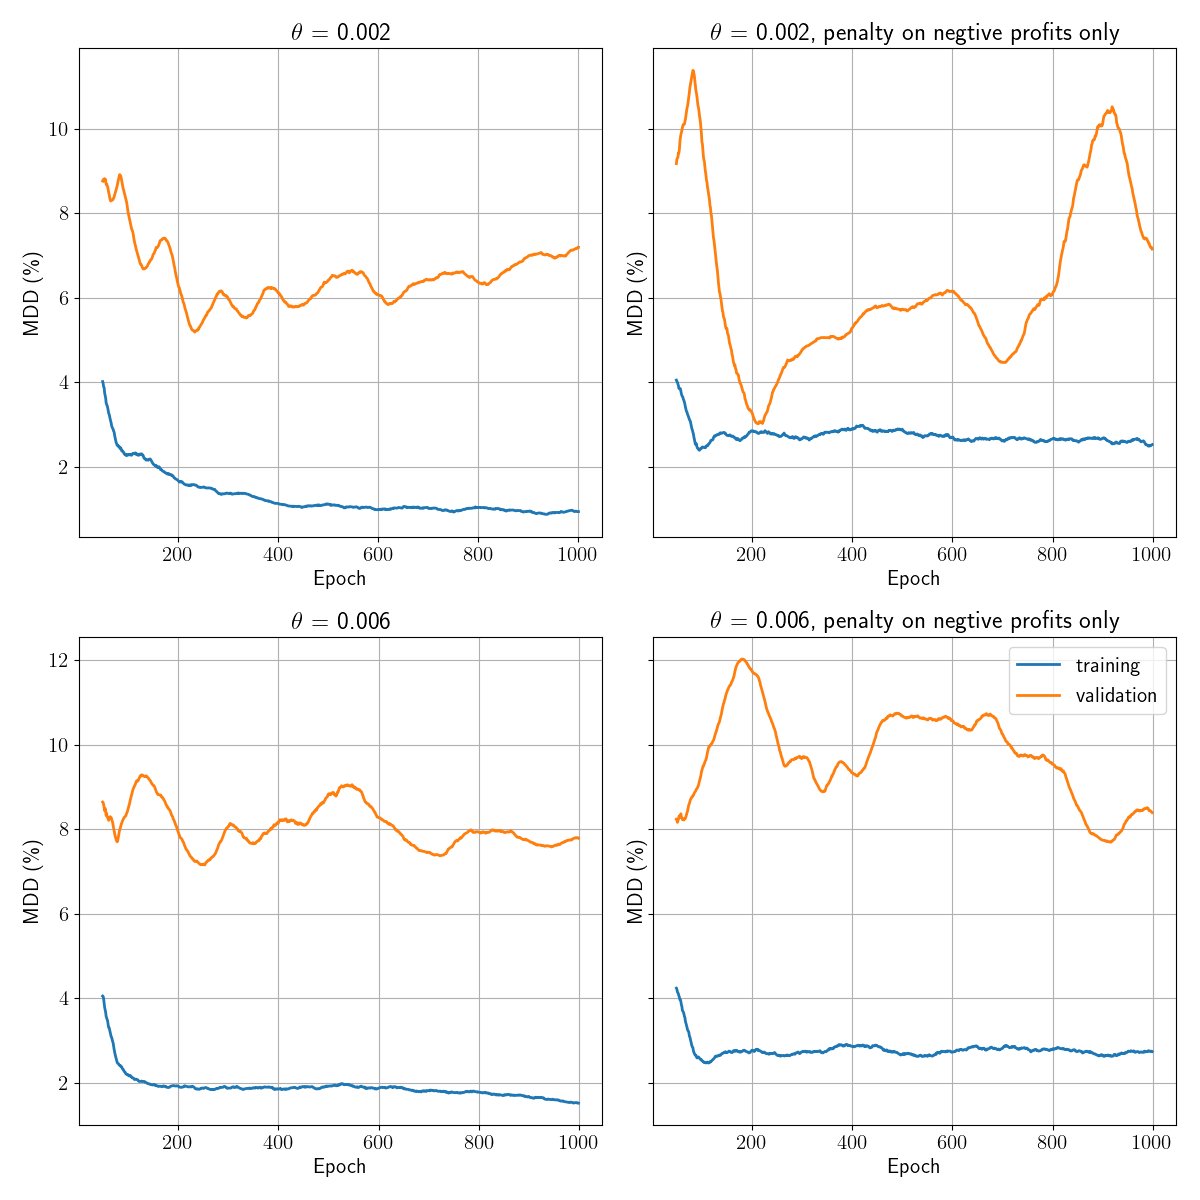
\includegraphics[width=15cm]{images/penalty_negtive_profits_compare.png}
  \caption [Comparison of penalty all profits and negative profits only] {Comparison of XXXXX in terms of training and validation MDD (moving average 50 epochs)}
  \label{fig:negtive_profits_diagram}
\end{figure}